\subsection{Reprezentace znalostí}\label{subsec:reprezentace_znalosti}
Pro porovnání obrázku s jeho popisem v přirozené řeči bylo nutné zvolit či navrhnout nějakou formu reprezentace znalostí,
která by umožnila zachytit sémantiku z obou zdrojů.
Jak již bylo výše zmíněno, zvolen byl expertní přístup a to v tomto případě znamená, že referenční popis obrázku je vytvořen lidským expertem,
což klade další omezení na formát reprezentace znalostí.
\todo{zmínit, že expertní přístup umožňuje lepší kontrolu nad obsahem/kvalitou než automat/statistika?}

Při návrhu bylo tedy potřeba brát v úvahu následující požadavky a najít nějaký formát, který by představoval vhodný kompromis mezi nimi.
\begin{itemize}
	\item \textbf{Čitelnost člověkem}:\\
	      Aby byl lidský expert schopen vytvořit, číst a případně upravit referenční popisy,
	      je nutné, aby byl schopen porozumět formě a zápisu uložených dat.
	      Toto omezení tedy upřednostňuje textové formáty a prakticky vyřazuje binární data.

	      Výjimku by mohl tvořit nějaký binární formát s přidruženým editorem,
	      kde by člověk mohl v grafickém prostředí prohlížet a manipulovat data, ale takový případ je nad rámec této práce.
	\item \textbf{Kompaktnost a struktura dat}:\\
	      Dalším důležitým aspektem je struktura a kompaktnost dat.
	      Pomocí počítače je poměrně snadné v krátkém čase zpracovat velké množství jednoduchých datových záznamů,
	      nicméně člověk se bude lépe orientovat v nějakém kompaktnějším popisu, který ačkoli může být složitější ve své struktuře,
	      tak bude pro člověka lépe názorný a uchopitelný.
	\item \textbf{Univerzálnost formátu}:\\
	      Podstatnou vlastností pro hledanou reprezentaci znalostí je její schopnost zachytit popis různých obrázků.
	      Navržený formát tedy musí být dostatečně univerzální, aby pomocí něj šlo popsat co nejširší spektrum informací,
	      od jednoduchých obrázků zobrazujících například jeden statický objekt, přes složitější obrázky zobrazující více objektů,
	      až po dynamické komplexní scény zobrazující mnoho objektů, činnosti a vazby mezi nimi.
	\item \textbf{Počítačová zpracovatelnost}:\\
	      V neposlední řadě je také potřeba dbát na to, aby navržený formát bylo možné co nejsnadněji zpracovat programově, na počítači.
	      Dynamické formáty s volnou strukturou bývají složitější na strojové zpracování, než fixní formáty s přesně definovanou podobou.
\end{itemize}

S ohledem na tyto body byla navržena reprezentace znalostí založená na sémantických sítích, která definuje 4 základní \emph{aspekty popisu}: objekty, jejich hierarchii,
statické atributy a dynamické vazby.
Detailnější popis těchto jednotlivých aspektů je v následujících částech, konkrétní technická implementace je pak popsána v sekci~\ref{sec:implementace}.
\todo{jak a kde se správně používá emph pro zdůraznění pojmu/termínu?}

\subsubsection{Objekty ve scéně}\label{subsubsec:objekty_ve_scene}
\newcommand{\objekt}{{\color{red!70!black}\texttt{objekt}}}
Cokoli, co lze v obrázku ohraničit rámečkem (angl.~bounding-box)
\todo{jak s anglikanismy?}
a při separaci od zbytku scény (obrázku) neztratí nebo zásadně nezmění svůj význam,
lze považovat za \emph{objekt}.

Jako \emph{objekt} v obrázku lze tedy označit zobrazené fyzické předměty, postavy, zvířata, ale také nehmotné pojmy jako \enquote{nebe},
místa, lokace či místnosti (např.~\enquote{kuchyň} nebo \enquote{louka}) a části jiných objektů (např.~\enquote{obličej} jsou součást hlavy nebo celého člověka).

Tato definice objektu byla záměrně navržena velmi obecně, aby byl definovaný formát univerzální a šel použít i pro popis velmi odlišných obrázků s různými účely.
Potenciální nevýhodou, která plyne z univerzálnosti formátu, může být v některých situacích problém nejednoznačnosti.

V jednom obrázku lze definovat různé množiny objektů, podle toho, jak moc detailní popis expert vytvoří.
Například pokud by byl na obrázku člověk, lze jej popsat jedním objektem jako \enquote{člověk} nebo \enquote{osoba},
ale také by šlo definovat ještě mnoho dalších objektů, například pro jednotlivé části těla nebo oblečení.

Kromě různých úrovní detailů lze také na problematiku nejednoznačnosti narazit v situaci, kdy je pro nějaký (dostatečně komplexní) obrázek
možné sestavit různé množiny objektů podle toho, pro jaké potřeby je zrovna obrázek a referenční popis používán.
Pro aplikaci, kde je podstatné zachycení živých objektů, může být množina objektů v referenčním popise tvořena lidmi či zvířaty.
Pro jiné použití pak ale může být podstatné zachytit prostředí a neživé předměty,
takže množina objektů by byla tvořena částmi prostředí (např.~stromy, křoví, voda, skály), budovami nebo obecnými předměty.
\todo{vyměnit dlouhé popisy za jeden ukázkový příklad?}

\subsubsection{Hierarchie objektů}
Kromě množiny samotných objektů lze v obrázku také definovat jejich hierarchii.
To přirozeně plyne z výše zmíněné definice \emph{objektu}, která umožňuje specifikovat část existujícího objektu jako další samostatné objekty.

Příkladem takového popisu může být například situace, kdy je na obrázku strom.
Strom je možné rozdělit na korunu a kmen, korunu pak je možné dále dělit na větve.
Schématicky lze tento popis znázornit jako stromovou strukturu, viz Obrázek~\ref{fig:schema_hierarchie_objektu}.
\begin{figure}[H]
	\centering
	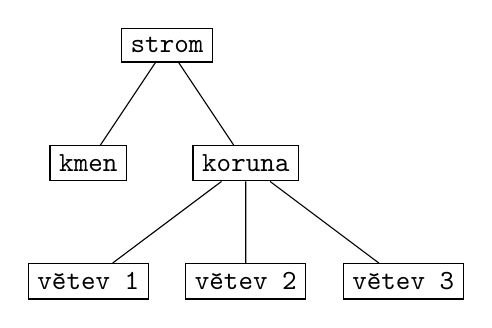
\begin{tikzpicture}[sibling distance=20mm]
		\node[draw, rectangle] {\texttt{strom}}
		child {node[draw, rectangle] {\texttt{kmen}}}
		child {node[draw, rectangle] {\texttt{koruna}}
				child {node[draw, rectangle] {\texttt{větev 1}}}
				child {node[draw, rectangle] {\texttt{větev 2}}}
				child {node[draw, rectangle] {\texttt{větev 3}}}
			}
		;
	\end{tikzpicture}
	\caption{Schématické znázornění hierarchie objektů}\label{fig:schema_hierarchie_objektu}
\end{figure}

Z pohledu daného objektu jsou \enquote{vyšší} (obecnější) objekty označované jako \emph{rodičovské objekty} (nebo jen \emph{rodiče}) a
\enquote{nižší} (konkrétnější) objekty pak jako \emph{potomci}.

Možnost definovat hierarchii objektů nabízí mimo jiné také způsob, jak vytvořit skupiny objektů, které k sobě nějakým způsobem patří.
Například strom může být součástí lesa, kráva může být součástí stáda nebo postava na hřišti může být součástí fotbalového týmu.
Tato příslušnost objektu nějaké skupině je dalším typem sémantické informace, kterou umožňuje navržený formát zachytit bez nutnosti definovat další specializované struktury.

Mohou však nastat situace, kdy je potřeba jeden objekt zařadit do několika různých skupin.
Z tohoto důvodu bylo rozhodnuto, že každý objekt může mít libovolné množství rodičů a libovolné množství potomků.
\todo{zdůvodňovat? dávat příklad? přirovnávat k OOP dědičnost vs kompozice?}

\subsubsection{Atributy objektů}
Vedle pouhého výčtu samotných objektů ve scéně je dále přirozeným požadavkem, aby byla reprezentace znalostí schopna zachytit i jejich vlastnosti.
K tomu slouží třetí aspekt popisu - \emph{atribut}.

Atributem je možné popsat jakoukoli informaci o objektu, která není závislá na jiném objektu.
Jinými slovy, pokud bychom objekt izolovali od zbytku scény (obrázku), tak všechny vlastnosti, které se tím nezmění nebo nezaniknou, lze popsat pomocí atributů.
Typickým příkladem je barva nebo tvar objektu či jeho části.
% Příkladem vlastnosti, která formulované definici atributu neodpovídá, je například velikost.
% To je z toho důvodu, že pokud bychom objekt izolovali od zbytku obrázku, ztrácíme informace o relativní velikosti oproti zbytku scény a nemůžeme již určit,
% zda je objekt \enquote{velký} či \enquote{malý}.

Atribut se skládá ze zvoleného \emph{názvu} a přiřazené \emph{hodnoty}, kdy konkrétní názvy a hodnoty jsou volbou experta, který tvoří referenční popis.
Název atributu označuje jakou vlastnost daný atribut popisuje a přiřazená hodnota pak udává, jaké konkrétní hodnoty nabývá.
Každý objekt může mít libovolné množství těchto atributů.

Názvy atributů pod jedním objektem nemusí být unikátní, lze specifikovat víc stejnojmenných atributů s různými hodnotami.
Typickým příkladem může být vícebarevný objekt, kde atribut s názvem \enquote{barva} bude vícekrát, pro různé konkrétní barvy.
Příklad jednoho takového popisu je na Obrázku~\ref{fig:example_tshirt}, kde název objektu je \enquote{tričko}
a definované jsou tři atributy: dvě barvy a vzor.
\todo{hezčí tabulka pro popis objektu?}
\todo{přidat šipky a popisky do tabulky co je co?}

\begin{figure}[H]
	\centering
	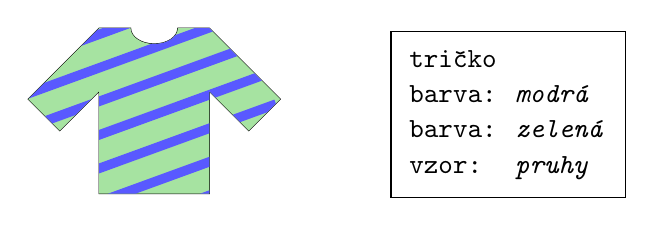
\begin{tikzpicture}
		\definecolor{green1}{HTML}{A6E3A1}
		\begin{scope}
			\draw[clip] (0,-1) -- ++(0.7,0) -- ++(0,1.3) -- ++(0.5,-0.5) -- ++(0.4,0.4) -- ++(-0.9,0.9) -- ++(-0.4,0)
			arc[start angle=0,end angle=-180,x radius=0.3, y radius=0.2]
			-- ++(-0.4,0) -- ++(-0.9,-0.9) -- ++(0.4,-0.4) -- ++(0.5,0.5) -- ++(0,-1.3) -- cycle;
			\begin{scope}[rotate=20]
				\draw[fill=green1,draw=none] (0,0) circle (2);
				\foreach \n in {0, 1, ..., 10}{
						\node[transform shape,scale=0.3,fill=blue!65,draw=none,minimum width=10cm, minimum height=4mm] at (0,-2+\n*0.4) {};
					}
			\end{scope}
		\end{scope}
		\matrix[draw, anchor=west] at (3, 0) {
			\node  {\texttt{\textbf{tričko}}};  \\
			\node {\texttt{barva:}}; &
			\node {\texttt{\textit{modrá}}};   \\
			\node {\texttt{barva:}}; &
			\node {\texttt{\textit{zelená}}};   \\
			\node {\texttt{vzor:}}; &
			\node {\texttt{\textit{pruhy}}};   \\
		};
	\end{tikzpicture}
	\caption{Příklad použití atributů pro popis objektu}\label{fig:example_tshirt}
\end{figure}

Pro složitější objekty se opět naskýtá problém toho, jaké vlastnosti vybrat a zapsat do referenčního popisu, a které je možné naopak zanedbat.
Tato otázka je podobná problematice nejednoznačnosti, zmíněné v části~\ref{subsubsec:objekty_ve_scene} definující objekty.
A i zde platí to, že popis byl záměrně vytvořen tak, aby byl univerzální a volba atributů do referenčního závisí na expertovi a konkrétní aplikaci.


\subsubsection{Vazby mezi objekty}
Posledním typem informace, kterou by měl být referenční popis obrázku schopen zachytit, jsou vazby a vztahy mezi různými objekty.
Může se jednat například o činnosti, které se týkají dvou objektů, nebo popis relativních vlastností, jako je velikost či pozice.

Každý takový záznam je označen jako \emph{triplet} a skládá se ze \emph{zdrojového objektu},
\emph{cílového objektu} a \emph{predikátu}, který popisuje danou vazbu nebo vztah.
Tato struktura je inspirována běžným zápisem sémantických sítí a RDF standardem.
\todo{doplnit reference!}
Obecné schéma jednoho tripletu je na Obrázku~\ref{fig:schema_tripletu}.

\begin{figure}[H]
	\centering
	\begin{tikzpicture}
		\node[draw, ellipse] (n1) at (0,0) {\texttt{zdrojový objekt}};
		\node[draw, ellipse] (n2) at (7,0) {\texttt{cílový objekt}};
		\draw[-Stealth] (n1) to node[midway, above] {\texttt{predikát}} (n2);
	\end{tikzpicture}
	\caption{Obecné schéma tripletu}\label{fig:schema_tripletu}
\end{figure}

Každý objekt může být součástí libovolného počtu tripletů a to jak v pozici zdrojového, tak cílového objektu.
Objekt také nemusí být součástí žádných vazeb a dokonce v celém popisu nemusí být žádné vazby definované.
Například pokud bychom chtěli pouze testovat paměť uživatele, mohli bychom mu ukázat obrázek, pak jej skrýt a sledovat, jaké objekty si vybaví.
V takové úloze nás vazby mezi objekty vůbec nemusejí zajímat a je tedy zbytečné, aby byly součástí referenčního popisu.

Při vytváření referenčního popisu obrázku se opět naskýtá otázka, jaké vazby a vztahy mezi objekty do popisu zavést a které lze ignorovat.
Například relativní velikost nebo pozice objektů může být pro některé úlohy klíčová, ale pro jiné zcela nepodstatná.
Tato problematika byla opět ponechána na expertovi, který vytváří referenční popis pro danou konkrétní aplikaci,
aby rozhodl, které informace je potřeba v referenčním popise zachytit.

Konkrétní příklad několika tripletů je znázorněn na Obrázku~\ref{fig:triplety_priklad}.
\begin{figure}[H]
	\centering
	\begin{tikzpicture}
		\node[draw] at (-5, 1) {
\includegraphics[scale=0.35]{imgs/dog_squirrel_tree_mushroom.pdf}};
		\node[draw, ellipse, minimum width=1.5cm, minimum height=1cm] (dog) at (0,0) {\texttt{pes}};
		\node[draw, ellipse, minimum width=2cm, minimum height=1cm] (sq) at (5,0) {\texttt{veverka}};
		\node[draw, ellipse, minimum width=2cm, minimum height=1cm] (tree) at (2,3) {\texttt{strom}};
		\node[draw, ellipse, minimum width=2cm, minimum height=1cm] (mush) at (5.5,3) {\texttt{houba}};
		\draw[-Stealth, bend left=25] (dog) to node[midway, above] {\footnotesize \texttt{běží za}} (sq);
		\draw[-Stealth] (dog) to node[midway, above] {\footnotesize \texttt{větší než}} (sq);
		\draw[-Stealth, bend left=25] (sq) to node[midway, below] {\footnotesize \texttt{utíká před}} (dog);
		\draw[-Stealth] (sq) -- node[midway, above, sloped] {\footnotesize \texttt{šplhá na}} (tree);
		\draw[-Stealth] (mush) -- node[midway, above, sloped] {\footnotesize \texttt{je pod}} (tree);
		\draw[-Stealth, bend left=30] (mush) -- node[midway, above, sloped] {\footnotesize \texttt{větší než}} (sq);
		\draw[-Stealth] (dog) to node[midway, above, sloped] {\footnotesize \texttt{je pod}} (tree);
	\end{tikzpicture}
	\caption{Příklad použití tripletů pro popis vztahů mezi objekty}\label{fig:triplety_priklad}
\end{figure}
\todo{příklad s kompletním popisem obrázku (všechno dohromady)?}
